\documentclass[conference]{IEEEtran}
\usepackage{cite}
\usepackage{amsmath,amssymb,amsfonts}
\usepackage{algorithmic}
\usepackage{graphicx}
\usepackage{textcomp}
\usepackage{xcolor}
\usepackage[printonlyused,withpage]{acronym}

\acrodefplural{DoF}[DoF]{degrees of freedom}
\acrodefplural{PM}[PM's]{pneumatic muscles}
\acrodefplural{PMA}[PMA's]{pneumatic muscle actuators}

\def\BibTeX{{\rm B\kern-.05em{\sc i\kern-.025em b}\kern-.08em
		T\kern-.1667em\lower.7ex\hbox{E}\kern-.125emX}}

\begin{document}
	
	\title{Simulation for a Two Degree of Freedom Robot Arm Actuated by Pneumatic Muscle Groups}
	
	\author{\IEEEauthorblockN{R. Nicholas Vandemark}
		\IEEEauthorblockA{\textit{University of Maryland} \\
			\textit{ENPM640 - Rehabilitation Robotics, Project}\\
			nickvand@umd.edu}
	}
	
	\maketitle
	
	\begin{abstract}
		Research on sliding-mode control techniques for a two degree of freedom planar robot arm actuated by pneumatic muscles is observed and discussed. Mathematical derivations for the robot model and control are described. A real-time capable simulation suite was developed and implementation details are discussed.
	\end{abstract}
	
	\begin{IEEEkeywords}
		Pneumatic muscle actuators, rehabilitative robotics, ROS2 simulation
	\end{IEEEkeywords}
	
	\section{Introduction}

	A \ac{PM} is an artifical bladder device whose expansion/contraction can be controlled via changes in pressure. It can induce actuation with many advantageous properties such as its light-weight and low cost materials, as well as its subsequent high power-to-weight ratio \cite{main-article}. Actuators that are comprised of \acp{PM} can be aptly referred to as a \ac{PMA}, and can be seen in antagonistic pairs when representing a system similar to a simple human joint. For example, a bicep and tricep muscle pair, which would represent two antagonist \acp{PM}, can act in opposing contraction and relaxation to actuate the corresponding elbow joint. Each "muscle" described here is more appropriately considered a "muscle group", where each group may also actually be comprised of many \acp{PM}, but together this muscle group creates a representation of a single e.g. bicep or tricep muscle. While in general it is not required, for the scope of this paper, each antagonistic muscle group (e.g. a bicep and tricep of a single \ac{PMA} segment) consist of the same number of \acp{PM}.

	Robotic systems which utilize \acp{PMA} can be implemented with numerous advantages in doing so. The benefits already mentioned would apply to each \ac{PMA} utilized in the system, but additionally, the structure of these \ac{PM} segments are likely more comfortable when interfacing with humans, such as in a rehabilitative exoskeleton \cite{main-article}. Standard mechatronic robotic segments would likely be heavier, harder, larger, and perhaps colder to the touch. All of these downsides introduce a rehabilitative device that could be less approachable for the user.

	The authors of \cite{main-article} discuss the history of robotic systems comprised of \acp{PMA}, as well as addresses control for a two \ac{DoF} planar robot arm. The hypothetical system consists of two robotic segments as described above, where each joint is actuated by antagnostic pairs of \acp{PM}, referred to there as a bicep and tricep muscle group. The reasoning for considering a sliding-mode control approach, above all other possible options, is also explained.

	This paper descibes an attempt at implementing a simulation for this hypothetical robotic system using \textit{ROS2} and \textit{MoveIt 2} according to the dynamic model described in \cite{main-article}, with fully dynamically configurable simulation parameters. Two cantral components were designed using the \textit{ros2\textunderscore control} framework, a custom controller which implements the sliding-mode control law, and a custom hardware interface which simulates reading/writing data from/to the robotic system.

	\section{Derivations and Calculations}

	As previously mentioned, a single segment for a robotic \ac{PMA} consists of two \ac{PM} groups, an example of which can be seen in Figure \ref{fig:pma_segment}, where the $b$ and $t$ subscripts denote a bicep and tricep muscle, respectively.

	\begin{figure}[htbp]
		\label{fig:pma_segment}
		\centerline{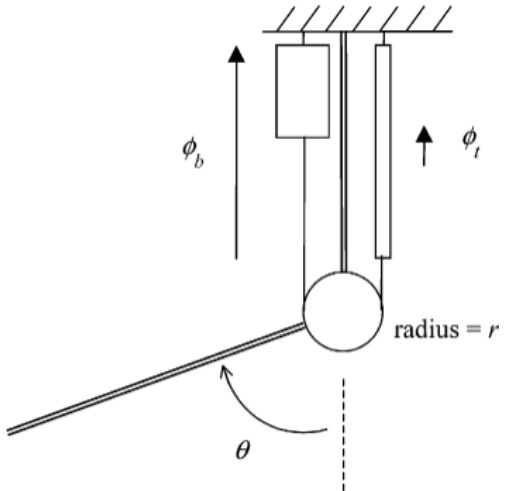
\includegraphics[width=\columnwidth]{images/pma.jpg}}
		\caption{Two \acp{PM} acting antagonistically to create a single robotic \ac{PMA} segment, Figure 2 of \cite{main-article}.}
	\end{figure}

	The force exerted by a \ac{PM} due to pressure change (i.e. expansion/contraction) is described by Eqn. \eqref{eq:force_pm}:

	\begin{equation}\label{eq:force_pm}
		\begin{aligned}
			\phi_{PM}(P, \theta, \dot{\theta}) = F_{PM}(P) &- K_{PM}(P) \cdot x_{PM}(\theta)\\
			&- B_{PM}(P) \cdot \dot{x}_{PM}(\dot{\theta})
		\end{aligned}
	\end{equation}

	where the force exerted by the \ac{PM} is a function of its current pressure and the position and velocity of the joint. The exact means to calculate the \ac{PM} length and lengthening rate ($x_{PM}(\theta)$ and $\dot{x}_{PM}(\dot{\theta})$, respectively) depend on the structure of the \ac{PM} segment, but is generally a function of the joint position and velocity. The nonlinear $F(P)$, $K(P)$, and $B(P)$ coefficients have expanded forms:
	
	\begin{equation}\label{eq:F_pm}
		F_{PM}(P) = F_{PM_{0}} + (F_{PM_{1}} \cdot P)
	\end{equation}
	
	\begin{equation}\label{eq:K_pm}
		K_{PM}(P) = K_{PM_{0}} + (K_{PM_{1}} \cdot P)
	\end{equation}
	
	\begin{equation}\label{eq:B_pm}
		B_{PM}(P) = \left\{
		\begin{aligned}
			B_{PM_{0_{i}}} + (B_{PM_{1_{i}}} \cdot P) & \text{  if PM is inflating} \\
			B_{PM_{0_{d}}} + (B_{PM_{1_{d}}} \cdot P) & \text{  else} \\
		\end{aligned}
		\right.
	\end{equation}

	The torque acting on the \ac{PM} segment due to this force is described by Eqn. \eqref{eq:torque_pm}:

	\begin{equation}\label{eq:torque_pm}
		\tau_{PM}(P, \theta, \dot{\theta}) = r_{PM} \cdot \phi_{PM}(P, \theta, \dot{\theta})
	\end{equation}

	where $r_{PM}$ is the radius of the pulley used in the \ac{PM} segment.

	The following is a more detailed and generalized derivation of Eqns. 3.6-3.7 from \cite{main-article}. The generalization is done so because it is how the simulation's code was implemented, and because it helps to showcase a possible reoccurring typo or unexplained simplification in this article. Consider what Lilly and Quesada stated (2004, p.351):

	\begin{quote}
		If several \acp{PM} are present in a system, each one generally has
		its own $F$, $K$, and $B$ coefficients, its own input pressure, and
		its own inflation or deflation status.
	\end{quote}

	which explicitly qualifies each \ac{PM} for its own unique characterization. The authors denote this with $b$ and $t$ subscripts in their Eqns. 2.7-2.8, but they are dropped for the $F$ and $K$ coefficients (but kept for the $B$ coefficient) starting with their Eqn. 3.1, but it does not seem to be explained as to why. Furthermore, according to their Eqns. 3.7a and 3.7c, if this were the case, then neither the values for $F_{0s}$ nor $K_{0s}$ would actually matter, as both of those terms are added and then subtracted out.

	For these reasons, it is believed to be best to generalize the equations to unique sets of coefficients for each \ac{PM} group (the shoulder bicep, shoulder tricep, elbow bicep, and elbow tricep).

	An input pressure for a \ac{PM} can be described as the sum of some positive nominal constant pressure and some offset from it, according to Eqn. \eqref{eq:input_pressure_pm}:
	
	\begin{equation}\label{eq:input_pressure_pm}
		P = P_{0} + \Delta p
	\end{equation}

	See Section IV of \cite{main-article} for a discussion on how this pressure for some \ac{PM} can be selected, such that the \ac{PMA} is well behaved in the absence of a control signal $\Delta p_{PM}$ and a desired joint stiffness is produced.

	The total torque acting on a \ac{PMA} pulley depends on how it is described. Figure \ref{fig:pma_robot_arm} shows that a torque due to the shoulder's tricep muscle is a positive contribution (and therefore the bicep muscle has a negative contribution), but that the elbow's tricep msucle is the negative contribution (and the bicep muscle is therefore the positive contribution). Furthermore, as mentioned previously, one e.g. 'bicep muscle' can also be respresented as a muscle group that consists of individual, identitical \acp{PM}. Considering all of this, combined with Eqn. \eqref{eq:torque_pm} produces Eqns. \eqref{eq:torque_pm_s} and \eqref{eq:torque_pm_e}, the torques acting on the shoulder and elbow \acp{PMA}, respectively:
	
	\begin{figure}[htbp]
		\label{fig:pma_robot_arm}
		\centerline{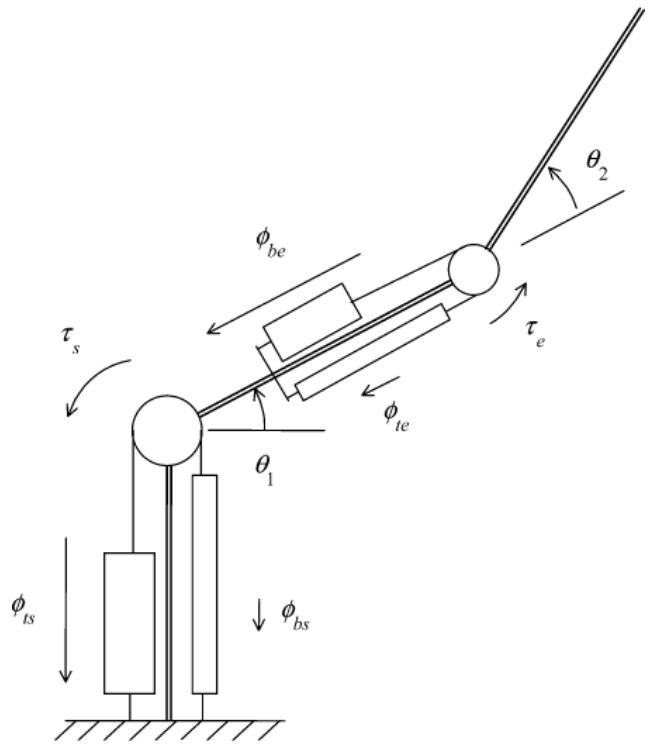
\includegraphics[width=\columnwidth]{images/two_dof_planar_pma_robot_arm.jpg}}
		\caption{Two \ac{DoF} planar robot arm with two \acp{PMA}, Figure 3 of \cite{main-article}.}
	\end{figure}
	
	\begin{equation}\label{eq:torque_pm_s}
		\tau_{s}(P_{b}, P_{t}) = n_{s} \cdot r_{s} \cdot \lbrack\phi_{s_{t}}(P_{t}) - \phi_{s_{b}}(P_{b}) \rbrack
	\end{equation}

	\begin{equation}\label{eq:torque_pm_e}
		\tau_{e}(P_{b}, P_{t}) = n_{e} \cdot r_{e} \cdot \lbrack\phi_{e_{b}}(P_{b}) - \phi_{e_{t}}(P_{t}) \rbrack
	\end{equation}

	where the forces due to \acp{PM} as part of the shoulder segment, $\phi_{s_{b}}(P)$ and $\phi_{s_{t}}(P)$, are a function of the first joint's position and velocity, and the forces due to \acp{PM} as part of the elbow segment, $\phi_{e_{b}}(P)$ and $\phi_{e_{t}}(P)$, are a function of the second joint's position and velocity.

	Assuming an input pressure to the shoulder bicep \ac{PM} $P_{bs} = P_{0bs} + \Delta p_{s}$ and an input to the shoulder tricep \ac{PM} $P_{ts} = P_{0ts} - \Delta p_{s}$, substituting this into Eqn. \eqref{eq:torque_pm_s} produces Eqn. \eqref{eq:torque_pm_s_sub_pressures_prereq}:

	\begin{equation}\label{eq:torque_pm_s_sub_pressures_prereq}
		\begin{aligned}
			\tau_{s}&(P_{b}=P_{0bs}+\Delta p_{s}, P_{t}=P_{0ts}-\Delta p_{s})\\
			&
			\begin{aligned}
				=&n_{s} \cdot r_{s} \cdot \lbrack F_{ts}(P_{0ts}-\Delta p_{s})-K_{ts}(P_{0ts}-\Delta p_{s}) \cdot x_{ts}\\
				&- B_{ts}(P_{0ts}-\Delta p_{s}) \cdot \dot{x}_{ts} \rbrack - \lbrack F_{bs}(P_{0bs}+\Delta p_{s})\\
				&-K_{bs}(P_{0bs}+\Delta p_{s}) \cdot x_{bs}-B_{bs}(P_{0bs}+\Delta p_{s}) \cdot \dot{x}_{bs} \rbrack
			\end{aligned}
		\end{aligned}
	\end{equation}

	Then, for each $F(P)$, $K(P)$, and $B(P)$ expression, make the substitution according to Eqns. \eqref{eq:F_pm}-\eqref{eq:B_pm} and group the $\Delta p_{PM}$ terms together, e.g.:
	
	\begin{equation}\label{eq:example_expand_sub_pressures}
		\begin{aligned}
			F_{ts}(P_{0ts}-\Delta p_{s}) &= F_{0ts} + (F_{1ts} \cdot (P_{0ts}-\Delta p_{s}))\\
			&= \lbrack -F_{1ts} \cdot \Delta p_{s} \rbrack + \lbrack F_{0ts} + F_{1ts} \cdot P_{0ts} \rbrack
		\end{aligned}
	\end{equation}

	Doing so for each produces Eqn. \eqref{eq:torque_pm_s_sub_pressures}:

	\begin{equation}\label{eq:torque_pm_s_sub_pressures}
		\begin{aligned}
			\tau_{s}&(P_{b}=P_{0bs}+\Delta p_{s}, P_{t}=P_{0ts}-\Delta p_{s}) = n_{s} \cdot r_{s} \cdot \lbrack\\
			&
			\begin{aligned}
				&\Delta p_{s} \cdot \lbrack -F_{1ts} + (x_{ts} \cdot K_{1ts}) + (\dot{x}_{ts} \cdot B_{1ts})\\
				&- F_{1bs} + (x_{bs} \cdot K_{1bs}) + (\dot{x}_{bs} \cdot B_{1bs}) \rbrack + F_{0ts}\\
				&+ (F_{1ts} \cdot P_{0ts}) - (x_{ts} \cdot (K_{0ts} + (K_{1ts}\cdot P_{0ts})))\\
				&- (\dot{x}_{ts} \cdot (B_{0ts} + (B_{1ts}\cdot P_{0ts}))) - F_{0bs}\\
				&- (F_{1bs} \cdot P_{0bs}) + (x_{bs} \cdot (K_{0bs} + (K_{1bs}\cdot P_{0bs})))\\
				&+ (\dot{x}_{bs} \cdot (B_{0bs} + (B_{1bs}\cdot P_{0bs}))) \rbrack
			\end{aligned}
		\end{aligned}
	\end{equation}

	Doing the same for Eqn. \eqref{eq:torque_pm_e} and assuming an input pressure to the elbow bicep \ac{PM} $P_{be} = P_{0be} + \Delta p_{e}$ and an input to the elbow tricep \ac{PM} $P_{te} = P_{0te} - \Delta p_{e}$ produces Eqn. \eqref{eq:torque_pm_e_sub_pressures}:
	
	\begin{equation}\label{eq:torque_pm_e_sub_pressures}
		\begin{aligned}
			\tau_{e}&(P_{b}=P_{0be}+\Delta p_{e}, P_{t}=P_{0te}-\Delta p_{e}) = n_{e} \cdot r_{e} \cdot \lbrack\\
			&
			\begin{aligned}
				&\Delta p_{e} \cdot \lbrack F_{1be} - (x_{be} \cdot K_{1be}) - (\dot{x}_{be} \cdot B_{1be})\\
				&+ F_{1te} - (x_{te} \cdot K_{1te}) - (\dot{x}_{te} \cdot B_{1te}) \rbrack + F_{0be}\\
				&+ (F_{1be} \cdot P_{0be}) - (x_{be} \cdot (K_{0be} + (K_{1be}\cdot P_{0be})))\\
				&- (\dot{x}_{be} \cdot (B_{0be} + (B_{1be}\cdot P_{0be}))) - F_{0te}\\
				&- (F_{1te} \cdot P_{0te}) + (x_{te} \cdot (K_{0te} + (K_{1te}\cdot P_{0te})))\\
				&+ (\dot{x}_{te} \cdot (B_{0te} + (B_{1te}\cdot P_{0te}))) \rbrack
			\end{aligned}
		\end{aligned}
	\end{equation}

	This is the derivation for Eqns. 3.6-3.7 from \cite{main-article}, but important to note is that these results do not agree. To put the findings here in that form would produce Eqns. \eqref{eq:torque_pm_s_simplified}-\eqref{eq:tau_1_e}:
	
	\begin{equation}\label{eq:torque_pm_s_simplified}
		\tau_{s}(P_{b}=P_{0bs}+\Delta p_{s}, P_{t}=P_{0ts}-\Delta p_{s}) = \tau_{0_{s}} + (\Delta p_{s} \cdot \tau_{1_{s}})
	\end{equation}

	\begin{equation}\label{eq:torque_pm_e_simplified}
		\tau_{e}(P_{b}=P_{0be}+\Delta p_{e}, P_{t}=P_{0te}-\Delta p_{e}) = \tau_{0_{e}} + (\Delta p_{e} \cdot \tau_{1_{e}})
	\end{equation}

	\begin{equation}\label{eq:tau_0_s}
		\begin{aligned}
			\tau_{0_{s}} = n_{s} \cdot r_{s} \cdot \lbrack & F_{0ts} + (F_{1ts} \cdot P_{0ts})\\
			&- (x_{ts} \cdot (K_{0ts} + (K_{1ts}\cdot P_{0ts})))\\
			&- (\dot{x}_{ts} \cdot (B_{0ts} + (B_{1ts}\cdot P_{0ts})))\\
			&- F_{0bs} - (F_{1bs} \cdot P_{0bs})\\
			&+ (x_{bs} \cdot (K_{0bs} + (K_{1bs}\cdot P_{0bs})))\\
			&+ (\dot{x}_{bs} \cdot (B_{0bs} + (B_{1bs}\cdot P_{0bs}))) \rbrack
		\end{aligned}
	\end{equation}

	\begin{equation}\label{eq:tau_1_s}
		\begin{aligned}
			\tau_{1_{s}} = n_{s} \cdot r_{s} \cdot \lbrack & - F_{1ts} + (x_{ts} \cdot K_{1ts}) + (\dot{x}_{ts} \cdot B_{1ts})\\
			&- F_{1bs} + (x_{bs} \cdot K_{1bs}) + (\dot{x}_{bs} \cdot B_{1bs}) \rbrack
		\end{aligned}
	\end{equation}

	\begin{equation}\label{eq:tau_0_e}
		\begin{aligned}
			\tau_{0_{e}} = n_{e} \cdot r_{e} \cdot \lbrack & F_{0be} + (F_{1be} \cdot P_{0be})\\
			&- (x_{be} \cdot (K_{0be} + (K_{1be}\cdot P_{0be})))\\
			&- (\dot{x}_{be} \cdot (B_{0be} + (B_{1be}\cdot P_{0be})))\\
			&- F_{0te} - (F_{1te} \cdot P_{0te})\\
			&+ (x_{te} \cdot (K_{0te} + (K_{1te}\cdot P_{0te})))\\
			&+ (\dot{x}_{te} \cdot (B_{0te} + (B_{1te}\cdot P_{0te}))) \rbrack
		\end{aligned}
	\end{equation}
	
	\begin{equation}\label{eq:tau_1_e}
		\begin{aligned}
			\tau_{1_{e}} = n_{e} \cdot r_{e} \cdot \lbrack & F_{1be} - (x_{be} \cdot K_{1be}) - (\dot{x}_{be} \cdot B_{1be})\\
			&+ F_{1te} - (x_{te} \cdot K_{1te}) - (\dot{x}_{te} \cdot B_{1te}) \rbrack
		\end{aligned}
	\end{equation}

	Eqns. \eqref{eq:tau_1_s} and \eqref{eq:tau_1_e} do not quite agree with Eqns. 3.7b and 3.7d from \cite{main-article}. Inspection of Eqns. \eqref{eq:force_pm} and \eqref{eq:F_pm}-\eqref{eq:B_pm} would reveal that the signs for the $K_{PM_{1}}$ and $B_{PM_{1}}$ terms must be the same for Eqns. \eqref{eq:tau_1_s} and \eqref{eq:tau_1_e}, which is the case here but not Eqns. 3.7b and 3.7d in \cite{main-article}. As such, it is believed the equations here are in the correct format.

	With these values derived, the sliding-mode control law can be implemented with an estimation of the sliding-mode gain matrix $G$ and vector $a$ using Eqns. 3.9 and 3.10 from \cite{main-article}, with the commanded pressures calculated via Eqn 5.10 from the same.

	\section{Simulation}

	Development began for a simulation suite which sits on top of the \textit{ROS2} framework, and more specifically, utilizes \textit{ros2\textunderscore control} and \textit{MoveIt 2}. \textit{ros2\textunderscore control} is a comprehensive hardware-agnostic framework for robotic control, which offers modular solutions for, among other things, trajectory control and simulated hardware interfaces, both of which were utilized for this project. \textit{MoveIt 2} is the robotic manipulation platform used to connect all the components in the simulation pipeline, including some boiler-plate functionality as well as the custom components designed specifically for this project.

	Figure \ref{fig:ros2_control_overview} shows an example, high-level block diagram of a system architecture such as this one. For this project, custom interfaces were designed to take the role of the ``arm\textunderscore controller'' and ``Simulation HW Interface'' blocks as seen in this diagram (though they have different command and state interfaces as the ones shown here, this is described in more detail in the upcoming sections).

	Unfortunately, while considerable progress was made on a full simulation suite for the type of robotic manipulator described in the previous sections, it could not be finished at this time. All algorithms have been implemented, and all \textit{ros2\textunderscore control} and \textit{MoveIt 2} connections have been made, but it does not perform as expected. In other words, there is a lingering bug in the design that could not be isolated in time. The following subsections describe the solutions attempted (including its current development state), as well as plans for future development.
	
	\begin{figure*}[htbp]
		\label{fig:ros2_control_overview}
		\centerline{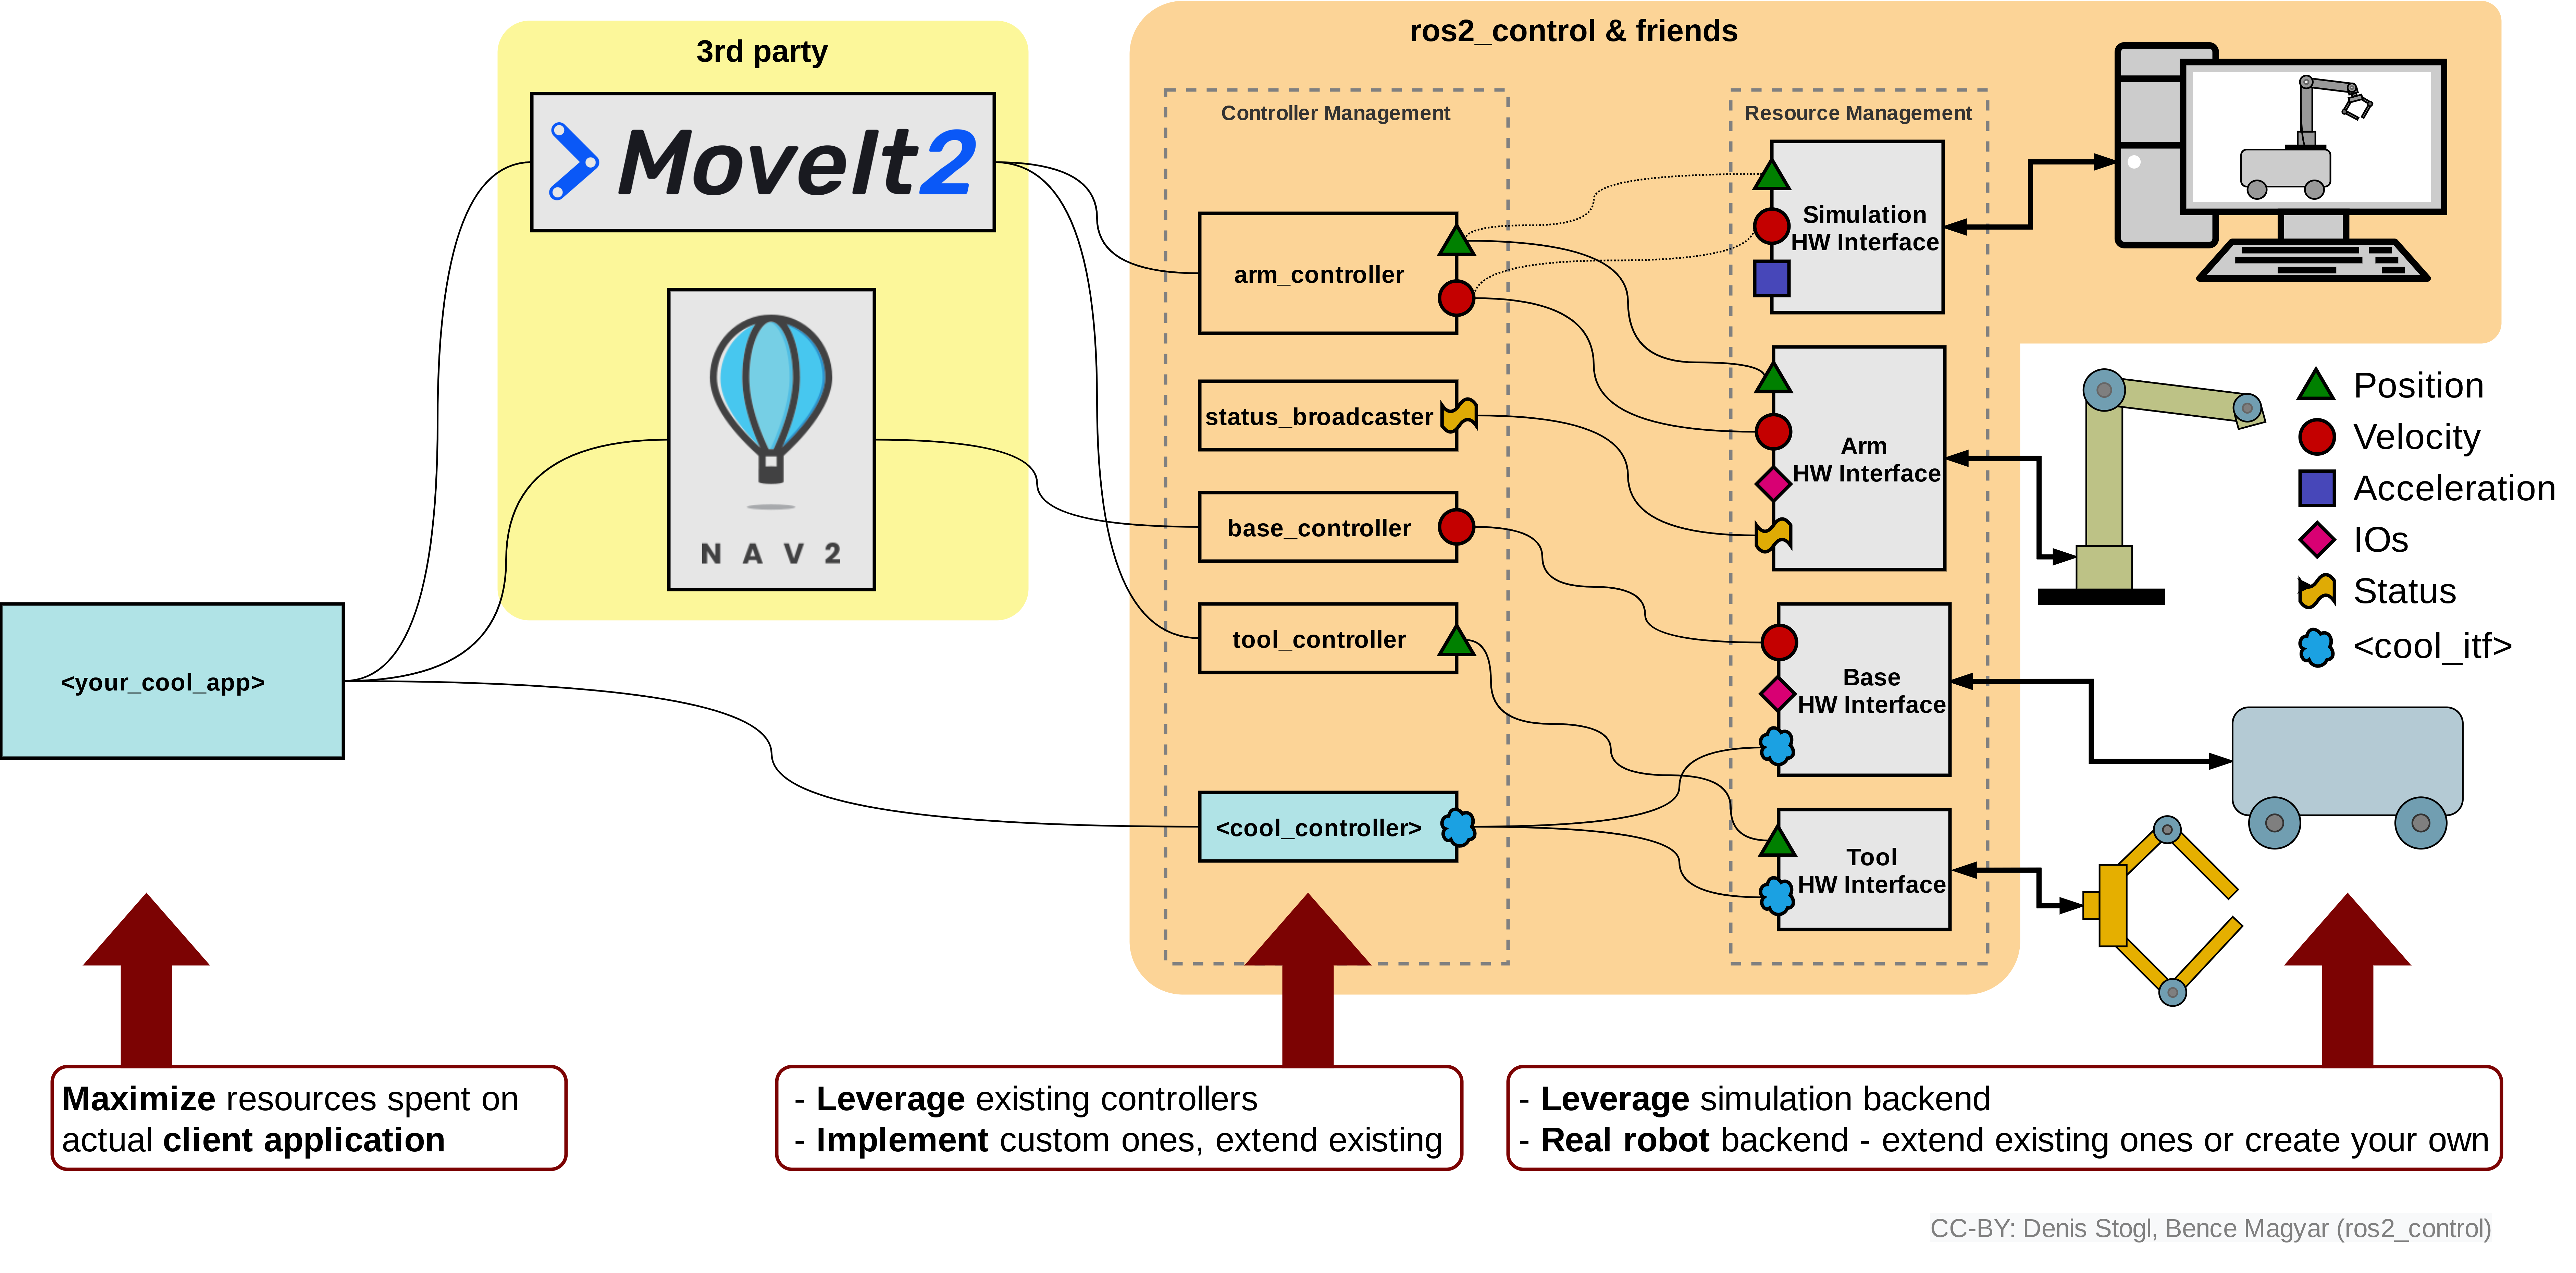
\includegraphics[width=2.0\columnwidth]{images/ros2_control_overview.png}}
		\caption{Overview of \textit{ros2\textunderscore control}. Source: \cite{ros2-control-overview}}
	\end{figure*}

	\subsection{Current Design}

	First, a URDF was created for a simple two \ac{DoF} planar arm, and the \textit{MoveIt Setup Assistant} was used to create a complete description of this robot model, such that it was ready to be used by \textit{MoveIt 2} (joint-space and Cartesian-space trajectory planning, simulated behavior, etc). From here, the runtime files could be updated to substitute custom \textit{ros2\textunderscore control} items as needed.

	Aside from various utilities to collect and publish trajectory control telemetry, maintain controller and \ac{PMA} segment configuration data, etc., the remainder of development went towards two custom \textit{ros2\textunderscore control} items, as described in the following subsections.

	\subsubsection{Custom Pressure-Trajectory Controller}

	The ``pressure-trajectory'' controller developed specifically for two \ac{DoF} planar robot arms consisting of \ac{PMA} segments uses the robot model and sliding-mode control algorithm described in \cite{main-article} to maintain the joint-space trajectory. This is where the above equations, as well as the relevant ones found in \cite{main-article}, are implemented. Once the next desired pressures are computed, the dynamics model is used one step further to calculate the joint accelerations that result from this (Eqn. 3.8 in \cite{main-article}), and these are what are commanded to the simulated hardware interface (see Section \ref{section:custom-hw-interface}).

	This \textit{ROS2} node also maintains a number of parameters via the \textit{ROS2} parameter server interface so the simulation is fully dynamically configurable. The parameters default to the ``ideal'' values as described in Section VI of \cite{main-article}, but are configurable on runtime so any desirable system configuration could be simulated. Their names and default values can be found in Tables \ref{table:control-sim-parameters} - \ref{table:pm-sim-parameters}.

	The design for this node was inspired by the joint trajectory controller offered by \textit{ros2\textunderscore control}, see those libraries for its implementation.

	\begin{table}
		\centering
		\begin{tabular}{|c|c|}
			\hline
			\textbf{Parameter Description} & \textbf{Default Value} \\\hline
			Acceleration due to gravity ($\frac{m}{s^2}$) & 9.81 \\\hline
			k1 sliding-mode control design constant (unitless) & 50.0 \\\hline
			k2 sliding-mode control design constant (unitless) & 50.0 \\\hline
			$\Gamma$1 sliding-mode control design constant (unitless) & 1.0 \\\hline
			$\Gamma$2 sliding-mode control design constant (unitless) & 1.0 \\\hline
			$\mu$1 sliding-mode control design constant (unitless) & 5.0 \\\hline
			$\mu$2 sliding-mode control design constant (unitless) & 5.0 \\\hline
		\end{tabular}
		\caption{Configurable simulation data for the sliding-mode controller and their default values.}
		\label{table:control-sim-parameters}
	\end{table}

	\begin{table}
		\centering
		\begin{tabular}{|c|c|}
			\hline
			\textbf{Parameter Description} & \textbf{Default Value} \\\hline
			shoulder segment mass (kg) & 10.0 \\\hline
			shoulder segment pulley radius (m) & 0.0762 \\\hline
			shoulder segment overall length (m) & 0.46 \\\hline
			shoulder segment length to CoM (m) & 0.23 \\\hline
			shoulder segment antagonist \ac{PM} pairs (count) & 6 \\\hline
			shoulder bicep nominal pressure (kPa) & 310.3 \\\hline
			shoulder tricep nominal pressure (kPa) & 449.6 \\\hline
		\end{tabular}
		\caption{Configurable simulation data for the robot shoulder segment and their default values.}
		\label{table:shoulder-segment-sim-parameters}
	\end{table}

	\begin{table}
		\centering
		\begin{tabular}{|c|c|}
			\hline
			\textbf{Parameter Description} & \textbf{Default Value} \\\hline
			elbow segment mass (kg) & 10.0 \\\hline
			elbow segment pulley radius (m) & 0.0508 \\\hline
			elbow segment overall length (m) & 0.46 \\\hline
			elbow segment length to CoM (m) & 0.23 \\\hline
			elbow segment antagonist \ac{PM} pairs (count) & 3 \\\hline
			elbow bicep nominal pressure (kPa) & 310.5 \\\hline
			elbow tricep nominal pressure (kPa) & 310.3 \\\hline
		\end{tabular}
		\caption{Configurable simulation data for the robot elbow segment and their default values.}
		\label{table:elbow-segment-sim-parameters}
	\end{table}

	\begin{table}
		\centering
		\begin{tabular}{|c|c|}
			\hline
			\textbf{Parameter Description} & \textbf{Default Value} \\\hline
			$F_{0}$ constant (unitless) & 179.2 \\\hline
			$F_{1}$ constant (unitless) & 1.39 \\\hline
			$K_{0}$ constant (unitless) & 5.71 \\\hline
			$K_{1}$ constant (unitless) & 0.0307 \\\hline
			$B_{0}$ constant (while inflating) (unitless) & 1.01 \\\hline
			$B_{1}$ constant (while inflating) (unitless) & 0.00691 \\\hline
			$B_{0}$ constant (while deflating) (unitless) & 0.6 \\\hline
			$B_{1}$ constant (while deflating) (unitless) & 0.000803 \\\hline
		\end{tabular}
		\caption{Configurable simulation data for each \ac{PM} (shoulder bicep, shoulder tricep, elbow bicep, and elbow tricep) and their default values.}
		\label{table:pm-sim-parameters}
	\end{table}

	\subsubsection{Custom Simulated PMA Robot Hardware Interface}\label{section:custom-hw-interface}

	This is a simple hardware interface which accepts commanded joint accelerations. The simulation is performed when ``reading'' the simulated
	acceleration by accepting the commanded value. The change in joint velocity and position is estimated given this change in acceleration, and the overall exposed state telemetry are the joint positions, velocities, and accelerations.

	The design for this node was inspired by a demo interface offered by \textit{ros2\textunderscore control}.

	\subsection{Attempted Design}\label{section:attempted-design}

	The initial design for this simulation suite also consisted of a custom trajectory controller and a custom hardware interface, but the state and command interface ``connections'' were different. One of the improvements made while designing the \textit{ros2\textunderscore control} utilities was that custom types of hardware interfaces could be defined. Its toolbox still comes with out-of-the-box solutions for common hardware interfaces (joint positions, velocities, and accelerations), as some combination of these are usually all that is needed for trajectory control for standard manipulators. But the ability to easily insert custom interfaces is also supported for outlier cases.

	For this project, it would have been more appropriate if this custom trajectory controller had a single command interface of type ``pressure'', in units of e.g. \textit{kPa}, for each joint in the \ac{PMA} robot arm. Then, the simulated hardware interface could simulate the system's response to such, and output joint positions, velocities, and accelerations according to its dynamics model. This leaves the ``pressure trajectory controller'' agnostic to the hardware interface that it is commanding pressures to, so a theoretical hardware interface for a physical version of a robot manipulator of this type could be swapped in for the simulated counterpart. The simulated hardware interface can simulate the state telemetry, while a physical hardware interface would measure it.

	There were issues with this approach that made implementation difficult on a timeline with a tight deadline. This is due largely to the way that robot hardware interfaces in \textit{ros2\textunderscore control} are not a node-based class and have limited communication with the \textit{ROS2} network, and simulating a response in this hardware interface without access to the additional metrics produced by the trajectory controller did not seem feasible.

	\subsection{Future Development}

	Future development would ideally be to revisit the original approach from Section \ref{section:attempted-design} and continuing that route for the custom trajectory controller and simulated hardware interface. Next step would be to find a solution to command Cartesian-space trajectories into \textit{MoveIt 2} that the custom trajectory controller can understand (i.e. \textit{MoveIt 2} automatically samples the trajectory in Cartesian-space and creates a corresponding one in joint-space, or the custom controller also caters to \textit{ROS2} Cartesian trajectory control and does the transformation to joint-space trajectories itself). From there, a simple node will listen to the telemetry output by the trajectory controller that is specific to \ac{PMA} robot models and plot the robot's trajectory in joint-space and ``pressure-space''.

	\section{Discussion and Conclusion}

	The theory and implementation described in \cite{main-article} was analyzed and summarized, and possible sources of human error throughout that article were discussed here. The model for a two \ac{DoF} planar robot arm consisting of segments actuated entirely by \acp{PM} was derived in a way that a sliding-mode trajectory controller could be designed for it. A simulation suite that utilizes \textit{ros2\textunderscore control} and \textit{MoveIt 2} was designed with some initial success, but has requires for development for a complete solution. A custom trajectory controller was developed specifically for a robot with the model discussed here, and a hardware interface was developed for the sake of simulating feedback. Other utilities were developed to support the full simulation pipeline.

	\section{List of Acronyms}

	\begin{acronym}
		\acro{DoF}{degree of freedom}
		\acro{PM}{pneumatic muscle}
		\acro{PMA}{pneumatic muscle actuator}
	\end{acronym}
	
	\begin{thebibliography}{00}
		\bibitem{main-article} J. H. Lilly and P. M. Quesada, ``A Two-Input Sliding-Mode Controller for a Planar Arm Actuated by Four Pneumatic Muscle Groups,'' IEEE Transactions on Neural Systems and Rehabilitation Engineering, vol. 12, no. 3, pp. 349--359, September 2004.
		\bibitem{ros2-control-overview} ros2\textunderscore control Maintainers,\\
		https://control.ros.org/master/doc/resources/resources.html, 2022.
	\end{thebibliography}
	
\end{document}
